% template adapted from https://github.com/jgm/pandoc-templates/blob/master/default.latex
%%%%%%%%%%%%%%%%%%%%%%%%%%%%%%%%%%%%%%%%%%%%%%%%%%%%%%%%%%%%%%%%%%%%%%%%%%%%%%%%%%%%%%%%%

% Options for packages loaded elsewhere
\PassOptionsToPackage{unicode=true}{hyperref}
\PassOptionsToPackage{hyphens}{url}
\PassOptionsToPackage{dvipsnames,svgnames*,x11names*}{xcolor}


\documentclass[
  11pt,
  french,
  a4paper,
  extrafontsizes,onecolumn,openright
  ]{memoir}

% Font family: lmodern by default
\usepackage{lmodern}

% Double (or whatever) spacing

\usepackage{amssymb, amsmath}
\usepackage{ifxetex,ifluatex}

% mathspec: arbitrary math fonts
\usepackage{unicode-math}
\defaultfontfeatures{Ligatures=TeX,Scale=MatchLowercase}

% More font families
% Main font
% Specific sanserif font
% Specific monotype font
% Specific math font
% Chinese, Japanese, Corean fonts

% Use upquote if available, for straight quotes in verbatim environments
\IfFileExists{upquote.sty}{\usepackage{upquote}}{}
% Use microtype if available
\IfFileExists{microtype.sty}{%
\usepackage[]{microtype}
\UseMicrotypeSet[protrusion]{basicmath} % disable protrusion for tt fonts
}{}

% Verbatim in note

\usepackage{xcolor}


% Geometry package

% Listings package



% Tables
\usepackage{longtable,booktabs,tabu}
% Fix footnotes in tables (requires footnote package)
\IfFileExists{footnote.sty}{\usepackage{footnote}\makesavenoteenv{longtable}}{}

% Graphics
\usepackage{graphicx,grffile}
\graphicspath{{images/}}
\makeatletter
\def\maxwidth{\ifdim\Gin@nat@width>\linewidth\linewidth\else\Gin@nat@width\fi}
\def\maxheight{\ifdim\Gin@nat@height>\textheight\textheight\else\Gin@nat@height\fi}
\makeatother
% Scale images if necessary, so that they will not overflow the page
% margins by default, and it is still possible to overwrite the defaults
% using explicit options in \includegraphics[width, height, ...]{}
\setkeys{Gin}{width=\maxwidth,height=\maxheight,keepaspectratio}



\setlength{\emergencystretch}{3em}  % prevent overfull lines
\providecommand{\tightlist}{%
  \setlength{\itemsep}{0pt}\setlength{\parskip}{0pt}}

\setcounter{secnumdepth}{5}

% set default figure placement to htbp
\makeatletter
\def\fps@figure{htbp}
\makeatother

% Include headers (preamble.tex) here
%%% Complete the preamble of the LaTeX template
%%%------------------------------------------------------------------------------

%%% Packages
\usepackage{lipsum} % Dummy text.
% Utilisation :
% Ajouter ici d'éventuels packages LaTeX


%%% Environnement "Essentiel" en début de chapitre
\usepackage[tikz]{bclogo}
\newenvironment{Essentiel}
  {\begin{bclogo}[logo=\bctrombone, noborder=true, couleur=lightgray!50]{L'essentiel}\parindent0pt}
  {\end{bclogo}}
% Utilisation :
%
%```{block, type='Essentiel'}
% Texte à mettre en valeur
% ```

%%% Blocs de code taille scriptsize
\let\oldverbatim\verbatim
\def\verbatim{\oldverbatim\scriptsize}
% Utilisation :
% S'applique aux blocs de code et résultats du code R
% opts_chunk$set(size="scriptsize") s'applique au code et ses résultats
% Si désaccord sur les résultats, \def\verbatim{...} est prioritaire


%%% Langues supplémentaires.
% Commenter pour désactiver, décommenter pour activer
% Référence: https://mirrors.chevalier.io/CTAN/macros/unicodetex/latex/polyglossia/polyglossia.pdf (table 3)
\usepackage{polyglossia}
% fr-FR
\setotherlanguage[]{french}
% Au choix: Anglais en-GB ou en-US (défaut)
%\setotherlanguage[variant=british]{english}
\setotherlanguage[]{english}
% pt-BR
%\setotherlanguage[variant=brazilian]{portuguese}
\usepackage{booktabs}
\usepackage{longtable}
\usepackage{array}
\usepackage{multirow}
\usepackage{wrapfig}
\usepackage{float}
\usepackage{colortbl}
\usepackage{pdflscape}
\usepackage{tabu}
\usepackage{threeparttable}
\usepackage{threeparttablex}
\usepackage[normalem]{ulem}
\usepackage{makecell}
\usepackage{xcolor}

\usepackage{enumitem}

\usepackage{polyglossia}
\setmainlanguage[]{french}


\usepackage[style=authoryear-ibid,backend=biber,citestyle=verbose-inote,pageref=true,isbn=false,backref=true,giveninits=true,uniquename=init,maxcitenames=2,maxbibnames=150,sorting=nyt,sortcites=false]{biblatex}
\addbibresource{Biblio1.bib}
\addbibresource{packages.bib}

% cslreferences environment required by pandoc > 2.7

% Specific commands for EcoFoG style. Must come after biblatex.
\usepackage{latex/BookTemplate}

% PDF title page to insert
\usepackage{pdfpages}

% Hyperref comes last
\usepackage{hyperref}
\hypersetup{
  pdftitle={Rapport de stage Edouard Sorin},
  pdfkeywords={Epidemiology, Machin learning, HLB = Huanglongbing, Partial Least Squares regression (PLS), Random Forests (RF), Remote sensing, Spectroscopy, Support Vector Machine (SVM)},
  colorlinks=true,
  linkcolor=Maroon,
  citecolor=Blue,
  urlcolor=Blue,
  breaklinks=true}

% Don't use monospace font for urls
\urlstyle{same}


% Title, author, etc. from YAML to LaTeX
%%%%%%%%%%%%%%%%%%%%%%%%%%%%%%%%%%%%%%%%%%%%%%%%%%%%%%%%%%

\title{Rapport de stage Edouard Sorin}


\author{true \and true \and true \and true}


\date{2021-06-14}


% Main title page with filigrane
%%%%%%%%%%%%%%%%%%%%%%%%%%%%%%%%%%%%%%%%%%%%%%%%%%%%%%%%%%

\newcommand{\MainTitlePage}[1][]{
	\SmallMargins % Margins
	\pagestyle{empty} % No header/footer
	~\\ % Print a character or the page will not exist
	\begin{textblock}{2}(30,10)
		\rule{1pt}{\paperheight-20mm}
	\end{textblock}
	\begin{textblock}{140}(50, 45)
		\flushright
		\begin{Spacing}{3}
			{\fontfamily{qtm}\selectfont\fontsize{45}{45}\selectfont \textsc{\thetitle}}
		\end{Spacing}
	\end{textblock}
	\begin{textblock}{140}(50, 125)
		\flushright
		{\fontfamily{qtm}\Large \theauthor}
	\end{textblock}
	\begin{textblock}{120}[1, 1](225, 297)
		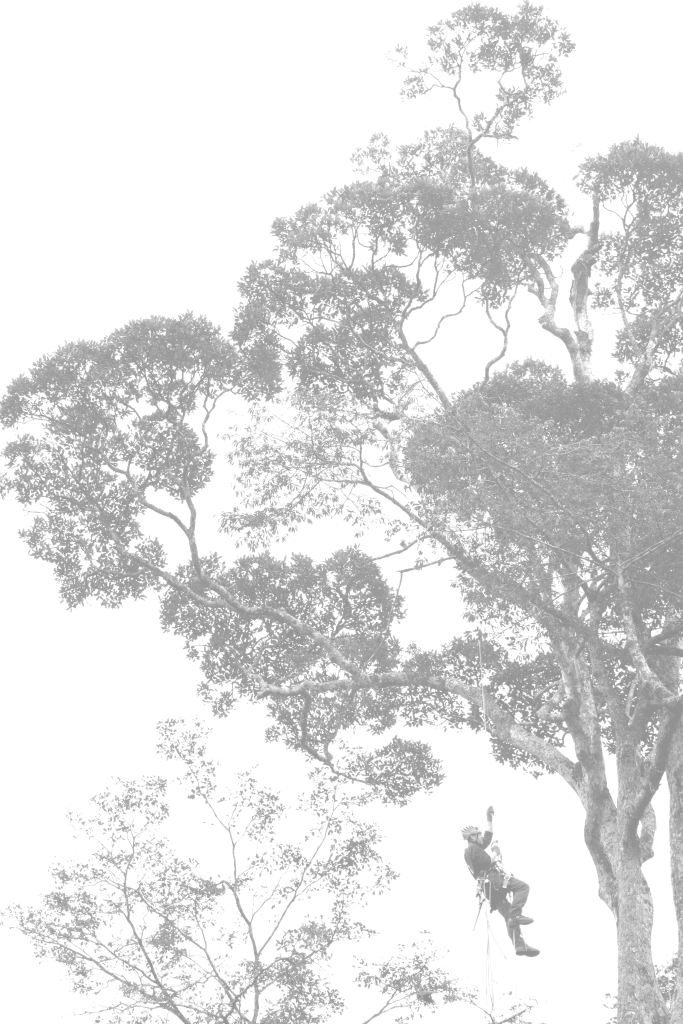
\includegraphics[width=10cm]{Filigrane}
	 \end{textblock}
	\begin{textblock}{140}[0, 1](50, 262)
		\normalfont	Version: \thedate
	\end{textblock}
	\newpage
	~\\ % Print a character or the page will not exist
	\begin{textblock}{140}(40, 40)
		#1
	\end{textblock}
	\begin{textblock}{140}[0,1](40, 270)
		\centering
    \includegraphics[width=5cm]{Logo-Lab}\\ \bigskip
		UMR \'Ecologie des forêts de Guyane\\
		\url{http://www.ecofog.gf}\\[3\baselineskip]
		Les opinions émises par les auteurs sont personnelles et n'engagent ni l'UMR EcoFoG ni ses tutelles.

    \tiny{Photographie en couverture: Hadrien Lalagüe}
	\end{textblock}
	\newpage
}


% End of preamble
%%%%%%%%%%%%%%%%%%%%%%%%%%%%%%%%%%%%%%%%%%%%%%%%%%%%%%%%%%


\begin{document}
\frontmatter

% Title page
%%%%%%%%%%%%%%%%%%%%%%%%%%%%%%%%%%%%%%%%%%%%%%%%%%%%%%%%%%

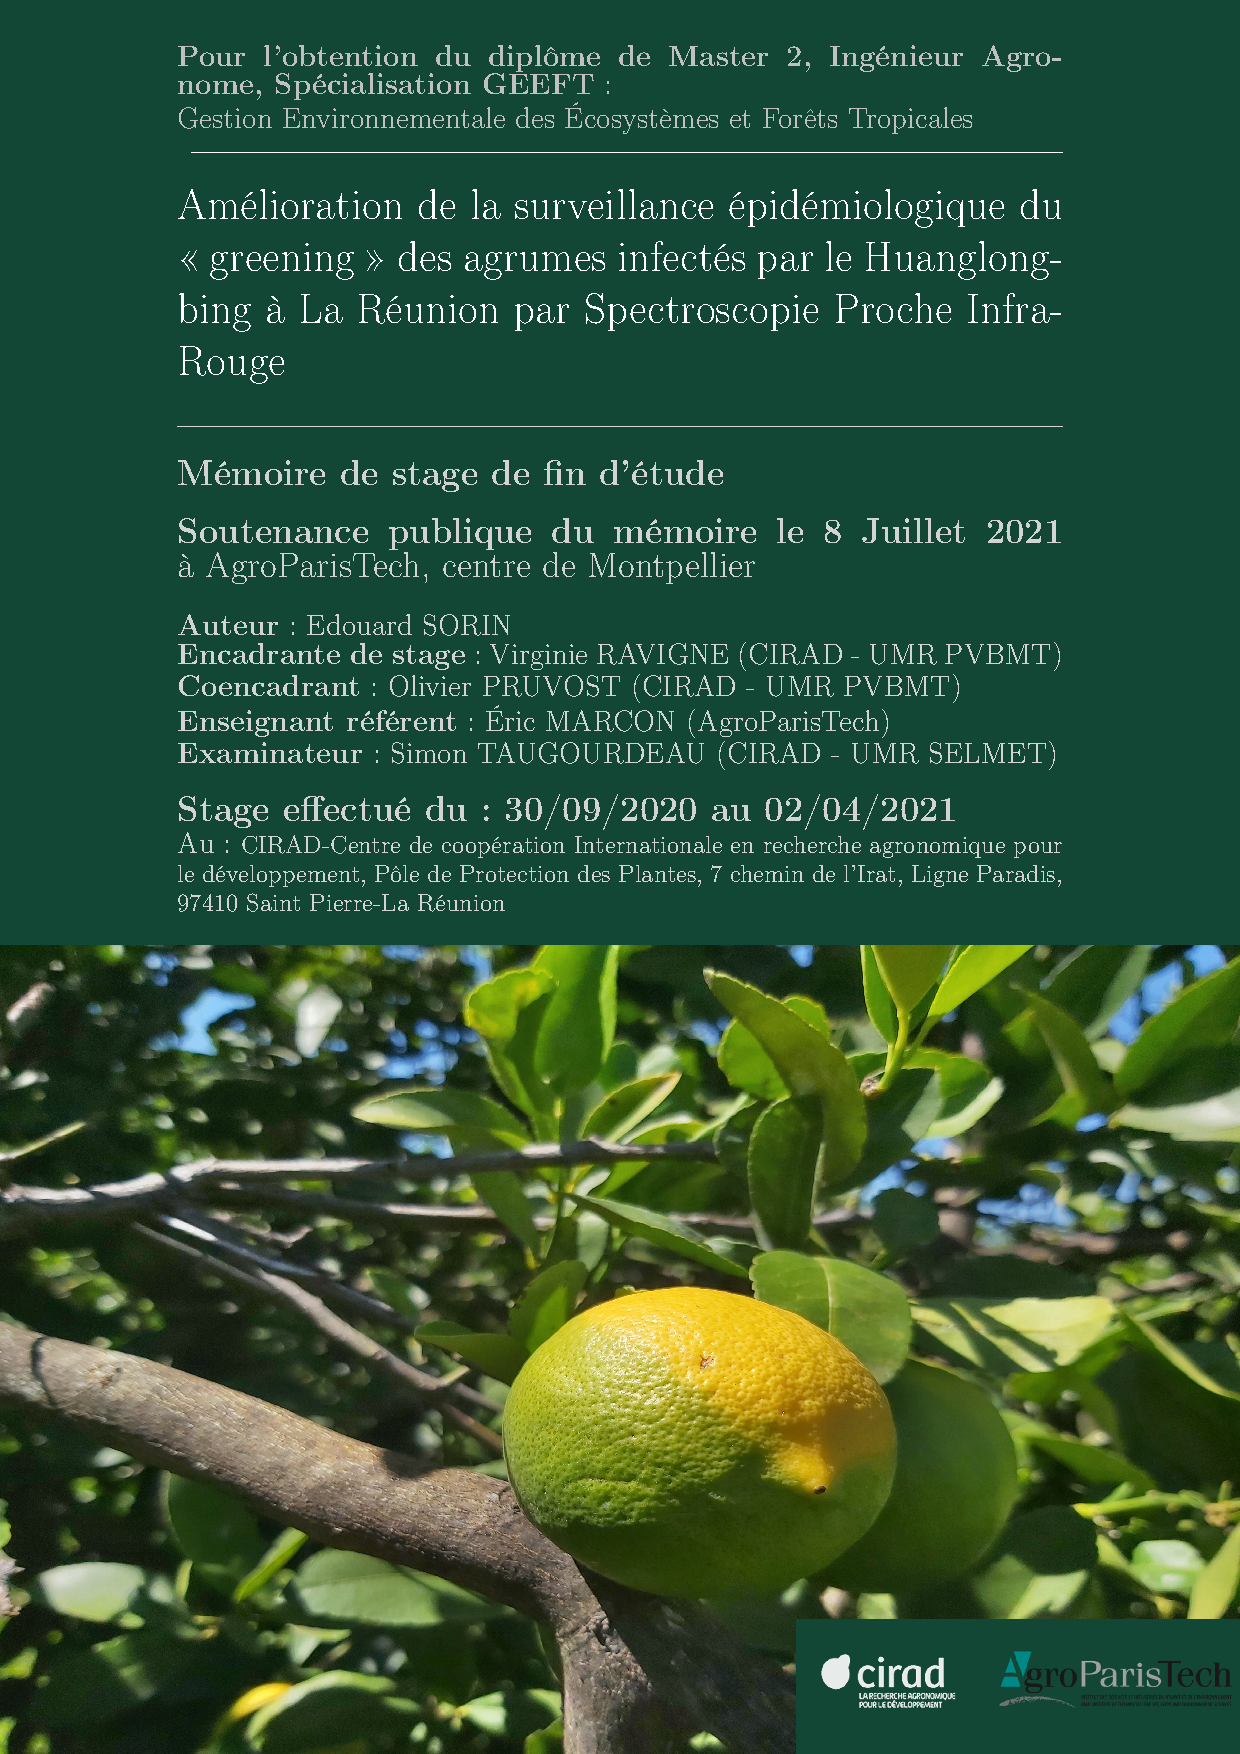
\includepdf[pages=1]{images/cover.pdf}
\cleardoublepage


% Resume/Abstract
%%%%%%%%%%%%%%%%%%%%%%%%%%%%%%%%%%%%%%%%%%%%%%%%%%%%%%%%%

\begin{description}

\selectlanguage{french}
\item[Résumé:]
Le \textbf{Huanglongbing (HLB)} est une maladie bactérienne causant le dépérissement des agrumes. Il y a une résurgence de cette maladie sur l'île de la Réunion depuis 2012, ce qui menace les vergers d'agrumes. Les techniques de détections classiques de surveillance de la maladie par PCR sont coûteuses, longues et ne peuvent pas être réalisées à grande échelle. C'est dans ce contexte qu'intervient la technologie de l'analyse par \textbf{imagerie spectrale}. Cette technologie se base sur l'analyse de la signature spectrale qu'émet un support en réponse à une exposition lumineuse. Cette méthode est non destructive pour le support traité, en plus d'être relativement peu coûteuse par rapport à la surface couverte. S'ajoute à cela un traitement des données d'imagerie spectrales par \textbf{apprentissage supervisé} dans le but de prédire le statut des arbres vis à vis de la maladie au sein des parcelles d'agrumes. Ce travail vise donc à améliorer la surveillance et la gestion de cette maladie en créant un modèle en apprentissage supervisé basé sur l'imagerie spectrale. Ce modèle est prometteur avec une qualité de la prédiction (Accuracy) de 92.6\% pour la méthode des Moindres Carrés Partiels (PLS) sur une base d'apprentissage de 8400 spectres de réflectance.

\selectlanguage{french}
\item[Mots clés :]
Apprentissage supervisé, Epidémiologie, Forêts Aléatoires (RF), HLB = Huanglongbing, Machine à Vecteurs de Support (SVM), Régression par les Moindres Carrés Partiels (PLS), Spectroscopie, Télédétection.
~\\
\vfill
\newpage
\selectlanguage{english}
\item[Abstract:]
\textbf{Huanglongbing (HLB)} is a bacterial disease causing dieback of citrus trees. There has been a resurgence of this disease on Reunion Island since 2012, which threatens citrus orchards. The conventional detection techniques for disease surveillance by PCR are expensive, time consuming and cannot be carried out on a large scale. This is where the technology of \textbf{spectral imaging} analysis comes in. This technology is based on the analysis of the spectral signature that a medium emits in response to light exposure. This method is non-destructive for the treated substrate, in addition to being relatively inexpensive compared to the surface covered. In addition, there is processing of spectral imaging data by \textbf{machine learning} in order to predict the status of trees with regard to disease within citrus plots. This work therefore aims to improve the surveillance and management of this disease by creating a supervised learning model based on spectral imaging. This model is promising with a prediction quality (Accuracy) of 92.6\% for the Partial Least Squares (PLS) method on a training base of 8400 reflectance spectra.

\selectlanguage{english}
\item[Keywords:]
Epidemiology, Machin learning, HLB = Huanglongbing, Partial Least Squares regression (PLS), Random Forests (RF), Remote sensing, Spectroscopy, Support Vector Machine (SVM).

\end{description}


% Before Body
%%%%%%%%%%%%%%%%%%%%%%%%%%%%%%%%%%%%%%%%%%%%%%%%%%%%%%%%%%





% Contents
%%%%%%%%%%%%%%%%%%%%%%%%%%%%%%%%%%%%%%%%%%%%%%%%%%%%%%%%%%

\LargeMargins
{
\hypersetup{linkcolor=}
\setcounter{tocdepth}{3}
\tableofcontents
}


% Body
%%%%%%%%%%%%%%%%%%%%%%%%%%%%%%%%%%%%%%%%%%%%%%%%%%%%%%%%%%

\LargeMargins
\hypertarget{remerciements}{%
\chapter*{Remerciements}\label{remerciements}}
\addcontentsline{toc}{chapter}{Remerciements}

Je tiens à remercier toutes les personnes qui ont contribué au bon déroulement de ce stage :

\begin{small}
\begin{itemize}

\item[——] Virginie RAVIGNE, mon encadrante de stage pour son encadrement, sa gentillesse , ses conseils et l'autonomie qu'elle m'a laissée au cours de ce stage afin que je développe mes propres axes de recherche sur cette thématique ;

\item[——] Frédéric CHIROLEU, chercheur en biostatistiques, co-auteur de ce rapport, et Thuy-Trang CAO, pour leur grande aide à la réalisation des scripts R et toutes les choses apprises lors de ces rendez-vous ;

\item[——] Olivier PRUVOST,  pour son aide lors des analyse qPCR et son encadrement au laboratoire ;

\item[——] Karine BOYER, pour m’avoir conseillé et formé aux techniques de laboratoire ;

\item[——] Ismaël HOUILLON, doctorant, pour ses conseils et ses jeux de mots douteux ;

\item[——] Elisa PAYET, technicienne à la FDGDON, pour avoir pris le temps de nous communiquer leurs résultats des détections du HLB et les numéros des agriculteurs ;

\item[——] Raphaël SOLESSE, ainsi que Emmanuel TILLARD, pour leurs conseils, sur le pilotage de drones et la formation à l’utilisation des instruments de mesure de spectrométrie ;

\item[——] Louis-Axel EDOUARD RAMBAUT, pour son aide sur les scripts R et ses discussions pertinentes ;

\item[——] Claire MELOT, stagiaire au CIRAD, pour sa bonne humeur et son aide aux analyses de laboratoire tardives ;

\item[——] Le CIRAD, l’équipe du 3P de Saint-Pierre et en particulier les agents de l’UMR PVBMT (Unité Mixte de 
Recherche Peuplements Végétaux et Bioagresseurs en Milieux Tropicaux) ;

\item[——] Les stagiaires des Kazz pour leur amitié, les mangues et toutes les choses partagées ensemble qui ont rendu ce stage inoubliable !

\end{itemize}
\end{small}

\mainmatter

\hypertarget{introduction}{%
\chapter{Introduction}\label{introduction}}

Placeholder

\hypertarget{contexte-guxe9nuxe9ral}{%
\section{Contexte général}\label{contexte-guxe9nuxe9ral}}

\hypertarget{etat-des-connaissances-sur-la-maladie}{%
\section{Etat des connaissances sur la maladie}\label{etat-des-connaissances-sur-la-maladie}}

\hypertarget{la-ruxe9surgence-du-hlb-uxe0-la-ruxe9union}{%
\section{La résurgence du HLB à la Réunion}\label{la-ruxe9surgence-du-hlb-uxe0-la-ruxe9union}}

\hypertarget{matuxe9riel-et-muxe9thodes}{%
\chapter{Matériel et Méthodes}\label{matuxe9riel-et-muxe9thodes}}

Placeholder

\hypertarget{identification-de-la-maladie}{%
\section{Identification de la maladie}\label{identification-de-la-maladie}}

\hypertarget{choix-des-arbres}{%
\section{Choix des arbres}\label{choix-des-arbres}}

\hypertarget{spectroscopie-uxe0-main}{%
\section{Spectroscopie à main}\label{spectroscopie-uxe0-main}}

\hypertarget{traitement-des-donnuxe9es-par-analyses-statistiques-et-apprentissage-supervisuxe9}{%
\section{Traitement des données par analyses statistiques et apprentissage supervisé}\label{traitement-des-donnuxe9es-par-analyses-statistiques-et-apprentissage-supervisuxe9}}

\hypertarget{foruxeats-aluxe9atoires-rf}{%
\section{Forêts Aléatoires (RF)}\label{foruxeats-aluxe9atoires-rf}}

\hypertarget{machine-uxe0-vecteurs-de-support-svm}{%
\section{Machine à Vecteurs de Support (SVM)}\label{machine-uxe0-vecteurs-de-support-svm}}

\hypertarget{ruxe9gression-par-les-moindres-carruxe9s-partiels-pls}{%
\section{Régression par les Moindres Carrés Partiels (PLS)}\label{ruxe9gression-par-les-moindres-carruxe9s-partiels-pls}}

\hypertarget{performance-des-classifications}{%
\section{Performance des classifications}\label{performance-des-classifications}}

\hypertarget{amuxe9lioration-du-protocole-de-terrain}{%
\section{Amélioration du protocole de terrain}\label{amuxe9lioration-du-protocole-de-terrain}}

\hypertarget{ruxe9sultats}{%
\chapter{Résultats}\label{ruxe9sultats}}

Placeholder

\hypertarget{influence-du-lieu-duxe9chantillonnage-et-des-variuxe9tuxe9s-sur-le-spectre-de-ruxe9flectance-global}{%
\section{Influence du lieu d'échantillonnage et des variétés sur le spectre de réflectance global}\label{influence-du-lieu-duxe9chantillonnage-et-des-variuxe9tuxe9s-sur-le-spectre-de-ruxe9flectance-global}}

\hypertarget{effet-du-statut-hlb-sur-les-spectres-de-ruxe9flectance}{%
\section{Effet du statut HLB sur les spectres de réflectance}\label{effet-du-statut-hlb-sur-les-spectres-de-ruxe9flectance}}

\hypertarget{lapproche-par-arbre-de-duxe9cision}{%
\section{L'approche par arbre de décision}\label{lapproche-par-arbre-de-duxe9cision}}

\hypertarget{comparaison-des-performances-des-3-muxe9thodes-de-pruxe9diction-du-statut-hlb-uxe0-partir-des-spectres-ruxe9flectance}{%
\section{Comparaison des performances des 3 méthodes de prédiction du statut HLB à partir des spectres réflectance}\label{comparaison-des-performances-des-3-muxe9thodes-de-pruxe9diction-du-statut-hlb-uxe0-partir-des-spectres-ruxe9flectance}}

\hypertarget{pruxe9diction-du-statut-hlb-par-ruxe9gression-par-les-moindres-carruxe9s-partiels-pls}{%
\section{Prédiction du statut HLB par Régression par les Moindres Carrés Partiels (PLS)}\label{pruxe9diction-du-statut-hlb-par-ruxe9gression-par-les-moindres-carruxe9s-partiels-pls}}

\hypertarget{amuxe9lioration-du-protocole-de-terrain-pour-le-choix-du-nombre-de-feuilles-par-arbre}{%
\section{Amélioration du protocole de terrain pour le choix du nombre de feuilles par arbre}\label{amuxe9lioration-du-protocole-de-terrain-pour-le-choix-du-nombre-de-feuilles-par-arbre}}

\hypertarget{amuxe9lioration-du-protocole-de-terrain-pour-le-choix-du-nombre-de-mesures-de-ruxe9flectance-par-feuille}{%
\section{Amélioration du protocole de terrain pour le choix du nombre de mesures de réflectance par feuille}\label{amuxe9lioration-du-protocole-de-terrain-pour-le-choix-du-nombre-de-mesures-de-ruxe9flectance-par-feuille}}

\hypertarget{annexe}{%
\chapter{Annexe}\label{annexe}}

Placeholder

\hypertarget{annexe-1-importation-des-donnuxe9es-brutes}{%
\section{Annexe 1 : Importation des données brutes}\label{annexe-1-importation-des-donnuxe9es-brutes}}

\hypertarget{annexe-2-fonction-matrice-de-confusion}{%
\section{Annexe 2 : Fonction Matrice de confusion}\label{annexe-2-fonction-matrice-de-confusion}}

\hypertarget{annexe-3-matrice-de-confusion-des-3-muxe9thodes-de-machin-learning}{%
\section{Annexe 3 : Matrice de confusion des 3 méthodes de machin learning}\label{annexe-3-matrice-de-confusion-des-3-muxe9thodes-de-machin-learning}}

\hypertarget{annexe-4-fonction-nombre-de-feuille}{%
\section{Annexe 4 : Fonction nombre de feuille}\label{annexe-4-fonction-nombre-de-feuille}}

\hypertarget{annexe-5-pruxe9diction-du-nombre-optimal-de-feuille}{%
\section{Annexe 5 : Prédiction du nombre optimal de feuille}\label{annexe-5-pruxe9diction-du-nombre-optimal-de-feuille}}

\hypertarget{annexe-6-fonction-nombre-de-ruxe9puxe9tition-spir-par-feuille}{%
\section{Annexe 6 : Fonction nombre de répétition SPIR par feuille}\label{annexe-6-fonction-nombre-de-ruxe9puxe9tition-spir-par-feuille}}

\hypertarget{annexe-7-pruxe9diction-du-nombre-de-ruxe9puxe9tition-optimal}{%
\section{Annexe 7 : Prédiction du nombre de répétition optimal}\label{annexe-7-pruxe9diction-du-nombre-de-ruxe9puxe9tition-optimal}}


% Bibliography
%%%%%%%%%%%%%%%%%%%%%%%%%%%%%%%%%%%%%%%%%%%%%%%%%%%%%%%%%%

\backmatter
\SmallMargins

%
\twocolumn
\renewcommand*{\bibfont}{\scriptsize}
\printbibliography
\onecolumn


% Tables (of tables, of figures)
%%%%%%%%%%%%%%%%%%%%%%%%%%%%%%%%%%%%%%%%%%%%%%%%%%%%%%%%%%




% After-body (LaTeX code inclusion)
%%%%%%%%%%%%%%%%%%%%%%%%%%%%%%%%%%%%%%%%%%%%%%%%%%%%%%%%%%




% Back cover
%%%%%%%%%%%%%%%%%%%%%%%%%%%%%%%%%%%%%%%%%%%%%%%%%%%%%%%%%%%

% Even page, small margins, no running head, no page number.
\evenpage
\SmallMargins
\thispagestyle{empty}

\begin{normalsize}


\end{normalsize}

\vspace*{\fill}
\centering\includegraphics[width=.7\textwidth]{images/Logo-Lab}
\end{document}
